% Source: printed p. 455; PDF p. 464
đẳng cấu của các tập hữu hạn $\sigma:m\xrightarrow{\cong}n$, trong đó $|m|=|n|$. Đặt $x=y\circ\sigma$; với mỗi $i\in n$, chú ý rằng $m_i=\sigma^{-1}(\{i\})=\{\sigma^{-1}(i)\}$, nên $x_i=x|_{\sigma^{-1}(i)}=y(i)$. Lấy $\id_{x_i}\in\mathcal O_{m_i}(x_i;y(i))$ với mỗi $i\in n$ và dùng luật đồng nhất, ta thấy công thức hợp thành cảm sinh một song ánh $\mathcal O_n(y;z)\xrightarrow{\cong}\mathcal O_m(x;z)$, có thể ký hiệu là
\stepcounter{equation}
\begin{equation}
\begin{aligned}
\sigma:\mathcal O(y(1),y(2),\ldots,y(n);z)\cong\qquad\\
\mathcal O\bigl(y(\sigma(1)),y(\sigma(2)),\ldots,y(\sigma(n));z\bigr).
\end{aligned}
\tag{7.18}
\end{equation}
Nói cách khác, nhóm hoán vị $\operatorname{Aut}(n)$ tác động lên tập $\mathcal O_n$ các cấu xạ $n$ ngôi bằng cách hoán vị thứ tự của các đối tượng miền $\Ob(\mathcal O)^n$.

Trong suốt cuốn sách, ta cho phép sự lạm dụng ký hiệu này và nói về các cấu xạ $\varphi:(y_1,y_2,\ldots,y_n)\to z$ với một số tự nhiên $n\in\mathbb N$, không nhắc đến sự lạm dụng vốn có trong việc chọn một thứ tự, miễn là rõ rằng hoán vị thứ tự các chỉ số sẽ không thay đổi gì tới đẳng cấu chính tắc ở~(7.18).

\noindent\textit{Ví dụ 7.4.1.3 (Operad các hình vuông nhỏ).}\keepwithnext
Một operad thường dùng trong toán học được gọi là \emph{operad các lập phương $n$ chiều nhỏ}. Ta tập trung vào $n=2$ và nói về \emph{operad các hình vuông nhỏ $\mathcal O$}. Ở đây tập các đối tượng chỉ có một phần tử, ký hiệu bằng một hình vuông, $\Ob(\mathcal O)=\{\square\}$. Với một số tự nhiên $n\in\mathbb N$, một cấu xạ $f:(\square,\square,\ldots,\square)\to\square$ là một cách đặt $n$ hình vuông không chồng nhau vào bên trong một hình vuông. Hình~7.5 minh họa một cấu xạ $(X_1,X_2,X_3)\to Y$, trong đó $X_1=X_2=X_3=Y=\square$.

Công thức hợp thành nói rằng cho một cách đặt những hình vuông nhỏ vào một hình vuông lớn, và cho một cách đặt những hình vuông tí hon vào mỗi hình vuông nhỏ ấy, ta được một cách đặt các hình vuông tí hon vào một hình vuông lớn. Xem Hình~7.6.

Ví dụ~7.4.1.3 minh họa tính tự đồng dạng được nhắc ở Mục~7.4.

\noindent\textit{Bài tập 7.4.1.4.}\keepwithnext
Xét một operad $\mathcal O$ giống operad các hình vuông nhỏ ở Ví dụ~7.4.1.3, nhưng có ba đối tượng: hình vuông, hình tròn và tam giác đều. Một cấu xạ vẫn là một cách đặt các hình không chồng nhau vào bên trong một hình.
\begin{enumerate}[label=\alph*.]
\item Vẽ một ví dụ về cấu xạ $f$ từ hai hình tròn và một hình vuông đến một tam giác.
\item Tìm ba cấu xạ khác hợp thành vào $f$, và vẽ hợp thành ấy.
\nobreak\hfill$\diamond$
\end{enumerate}

% Source: printed p. 456; PDF p. 465
\noindent\textit{Lời giải 7.4.1.4.}\keepwithnext
\begin{enumerate}[label=\alph*.]
\item
\begin{minipage}[t]{\linewidth}
\vspace{0pt}\centering
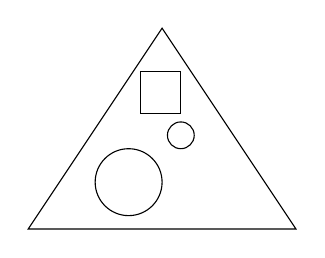
\begin{tikzpicture}[scale=.85]
\draw(0,0)--(4,0)--(2,3)--cycle;\draw(1.68,1.72)rectangle(2.28,2.35);\draw(2.28,1.4)circle(.2);\draw(1.5,.7)circle(.5);
\end{tikzpicture}
\end{minipage}
\item
\begin{minipage}[t]{\linewidth}
\vspace{0pt}\centering
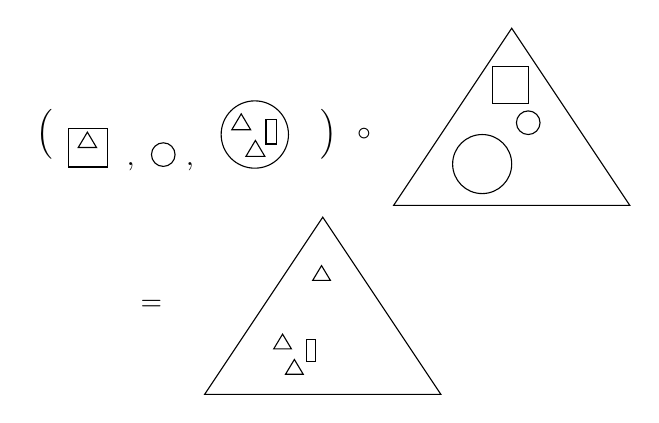
\begin{tikzpicture}[scale=.75,font=\normalsize]
\node at(-.7,1.2){$\Bigl($};\node at(4.1,1.2){$\Bigr)$};
\draw(-.3,.65)rectangle(.35,1.3);\draw(-.14,.98)--(.17,.98)--(.015,1.24)--cycle;
\node at(.75,.65){,};\draw(1.3,.86)circle(.2);\node at(1.75,.65){,};
\draw(2.85,1.2)circle(.57);\draw(2.46,1.28)--(2.78,1.28)--(2.62,1.55)--cycle;\draw(2.7,.83)--(3.02,.83)--(2.86,1.1)--cycle;\draw(3.04,1.04)rectangle(3.22,1.45);
\node at(4.7,1.2){$\circ$};
\begin{scope}[shift={(5.2,0)}]
\draw(0,0)--(4,0)--(2,3)--cycle;\draw(1.68,1.72)rectangle(2.28,2.35);\draw(2.28,1.4)circle(.2);\draw(1.5,.7)circle(.5);
\end{scope}
\node at(1.1,-1.7){$=$};
\begin{scope}[shift={(2,-3.2)}]
\draw(0,0)--(4,0)--(2,3)--cycle;\draw(1.83,1.93)--(2.13,1.93)--(1.98,2.18)--cycle;
\draw(1.17,.77)--(1.47,.77)--(1.32,1.02)--cycle;\draw(1.37,.34)--(1.67,.34)--(1.52,.59)--cycle;\draw(1.72,.56)rectangle(1.88,.93);
\end{scope}
\end{tikzpicture}
\end{minipage}
\nobreak\hfill$\blacklozenge$
\end{enumerate}

\noindent\textit{Ví dụ 7.4.1.5.}\keepwithnext
Cho $\mathbf{Sets}$ ký hiệu operad được định nghĩa như sau. Về đối tượng, đặt $\Ob(\mathbf{Sets})=\Ob(\Set)$. Với một số tự nhiên $n\in\mathbb N$ và các tập $X_1,\ldots,X_n,Y$, đặt
\[
\Hom_{\mathbf{Sets}}(X_1,\ldots,X_n;Y):=\Hom_{\Set}(X_1\times\cdots\times X_n,Y).
\]
% Source: printed p. 457; PDF p. 466
Cho các hàm $f_1:(X_{1,1}\times\cdots\times X_{1,m_1})\to Y_1$ đến $f_n:(X_{n,1}\times\cdots\times X_{n,m_n})\to Y_n$ và một hàm $Y_1\times\cdots\times Y_n\to Z$, tính chất phổ dụng cho một hàm duy nhất có dạng $(X_{1,1}\times\cdots\times X_{n,m_n})\to Z$, từ đó cho công thức hợp thành trong $\mathbf{Sets}$.

\subsubsection*{7.4.1.6\quad Operad: hàm tử và đại số}
Nếu operad giống phạm trù, ta có thể định nghĩa những thứ giống hàm tử và gọi chúng là \emph{hàm tử operad}.

\noindent\textit{Cảnh báo 7.4.1.7.}\keepwithnext
Thứ được gọi là hàm tử operad trong Định nghĩa~7.4.1.8 thường được gọi là \emph{cấu xạ operad}. Tôi cho rằng việc trùng thuật ngữ giữa cấu xạ \emph{của} các operad và cấu xạ \emph{trong} một operad gây nhầm lẫn. Điều này giống như điều sẽ xảy ra trong lý thuyết phạm trù thông thường (xem Chương~5) nếu ta thay từ \emph{hàm tử} bằng từ \emph{cấu xạ phạm trù}.

\noindent\textbf{Định nghĩa 7.4.1.8.}\keepwithnext
Cho $\mathcal O$ và $\mathcal O'$ là các operad. Một \emph{hàm tử operad từ $\mathcal O$ đến $\mathcal O'$}, ký hiệu $F:\mathcal O\to\mathcal O'$, được định nghĩa như sau. Ta công bố một số thành phần (A. phần trên đối tượng, B. phần trên cấu xạ) và chứng minh chúng tuân theo một số luật (1. bảo toàn đồng nhất, 2. bảo toàn hợp thành). Cụ thể, ta công bố
\begin{enumerate}[label=\Alph*.]
\item một hàm $\Ob(F):\Ob(\mathcal O)\to\Ob(\mathcal O')$, đôi khi chỉ ký hiệu là $F:\Ob(\mathcal O)\to\Ob(\mathcal O')$;
\item với mỗi đối tượng $y\in\Ob(\mathcal O)$, tập hữu hạn $n\in\Ob(\mathbf{Fin})$ và tập đối tượng có chỉ số trong $n$, $x:n\to\Ob(\mathcal O)$, một hàm
\[
F_n:\mathcal O_n(x;y)\longrightarrow\mathcal O'_n(Fx;Fy).
\]
\end{enumerate}
Sau đó phải chứng minh các \emph{luật hàm tử operad} sau đúng:
\begin{enumerate}[label=\arabic*.]
\item Với mỗi đối tượng $x\in\Ob(\mathcal O)$, phương trình $F(\id_x)=\id_{Fx}$ đúng.
\item Cho $s:m\to n$ là một cấu xạ trong $\mathbf{Fin}$. Cho $z\in\Ob(\mathcal O)$ là một đối tượng, $y:n\to\Ob(\mathcal O)$ là một tập các đối tượng có chỉ số trong $n$, và $x:m\to\Ob(\mathcal O)$ là một tập các đối tượng có chỉ số trong $m$. Khi ấy, với ký hiệu như trong Định nghĩa~7.4.1.1, sơ đồ các tập hợp sau giao hoán:
\stepcounter{equation}
\begin{equation}
\begin{tikzcd}[column sep=large,row sep=large,font=\scriptsize]
\mathcal O_n(y;z)\times\prod_{i\in n}\mathcal O_{m_i}(x_i;y(i))\arrow[r,"F"]\arrow[d,"\circ"']&\mathcal O'_n(Fy;Fz)\times\prod_{i\in n}\mathcal O'_{m_i}(Fx_i;Fy(i))\arrow[d,"\circ"]\\
\mathcal O_m(x;z)\arrow[r,"F"']&\mathcal O'_m(Fx;Fz)
\end{tikzcd}
\tag{7.19}
\end{equation}
\end{enumerate}
% Source: printed p. 458; PDF p. 467
Ta ký hiệu phạm trù các operad và các hàm tử operad là $\mathbf{Oprd}$.

\noindent\textit{Bài tập 7.4.1.9.}\keepwithnext
Cho $\mathcal O$ ký hiệu operad các hình vuông nhỏ ở Ví dụ~7.4.1.3, và cho $\mathcal O'$ ký hiệu operad các hình nhỏ mà bạn đã xây dựng trong Bài tập~7.4.1.4.
\begin{enumerate}[label=\alph*.]
\item Bạn có thể tìm một hàm tử operad $F:\mathcal O\to\mathcal O'$ không?
\item Có thể tìm một hàm tử operad $G:\mathcal O'\to\mathcal O$ không?
\nobreak\hfill$\diamond$
\end{enumerate}

\noindent\textit{Lời giải 7.4.1.9.}\keepwithnext
\begin{enumerate}[label=\alph*.]
\item Có. Một trong các hình thuộc $\Ob(\mathcal O')$ là hình vuông, nên ta biết $F$ trên đối tượng. Một cấu xạ trong $\mathcal O$ là một cách vẽ các hình vuông trong một hình vuông; đặc biệt, đây là một cách vẽ các hình trong một hình, nên có thể gán nó cho một cấu xạ trong $\mathcal O'$. Công thức hợp thành hoạt động đúng, nên ta đã định nghĩa được hàm tử operad.
\item Tôi không nghĩ ra một hàm tử như vậy. Nếu bạn nghĩ mình có một hàm tử, hãy cẩn thận nếu đang dùng bất kỳ phép thay đổi kích thước hay co giãn nào. Hãy nghĩ xem sự thay đổi kích thước đó tương tác thế nào với yêu cầu hàm tử phải bảo toàn các cấu xạ đồng nhất.
\nobreak\hfill$\blacklozenge$
\end{enumerate}

\noindent\textbf{Định nghĩa 7.4.1.10 (Đại số operad).}\keepwithnext
Cho $\mathcal O$ là một operad, và cho $\mathbf{Sets}$ là operad ở Ví dụ~7.4.1.5. Một \emph{đại số trên $\mathcal O$} là một hàm tử operad $A:\mathcal O\to\mathbf{Sets}$.

\noindent\textit{Nhận xét 7.4.1.11.}\keepwithnext
Có thể xem mỗi phạm trù là một operad (có một hàm tử $\Cat\to\mathbf{Oprd}$), trong đó mọi cấu xạ đều một ngôi. Nghĩa là, cho một phạm trù $\mathcal C$, ta tạo một operad $\mathcal O$ với $\Ob(\mathcal O):=\Ob(\mathcal C)$ và
\[
\Hom_{\mathcal O}(x_1,\ldots,x_n;y)=\begin{cases}\Hom_{\mathcal C}(x_1,y)&\text{nếu }n=1,\\\varnothing&\text{nếu }n\ne1.\end{cases}
\]
Trong suốt sách, ta liên hệ lược đồ cơ sở dữ liệu với phạm trù (xem Mục~5.2.2), theo đó một lược đồ $\mathcal C$ được xem là một trình bày phạm trù, tức bằng các phần tử sinh và các quan hệ. Tương tự, có thể bàn về các trình bày operad $\mathcal O$, cũng bằng phần tử sinh và quan hệ. Theo phép tương tự này, một thể hiện $\mathcal C\to\Set$ của cơ sở dữ liệu (xem Mục~5.2.2.6) tương ứng với một đại số $\mathcal O\to\mathbf{Sets}$ của operad.

% Source: printed p. 459; PDF p. 468
\subsection{Ứng dụng của operad và đại số của chúng}
Operad dường như mô hình hóa tốt các cấu trúc phân cấp. Một cấu trúc phân cấp thường có những khối xây dựng cơ bản cùng chỉ dẫn cách ghép chúng thành những khối lớn hơn. Mô tả các cấu trúc ấy bằng operad và đại số của chúng cho phép phân biệt thích hợp giữa các kiểu suy nghĩ khác nhau mà nếu không có thể bị lẫn lộn. Chẳng hạn, những chỉ dẫn xây dựng trừu tượng nên được mã hóa trong operad, còn các khối xây dựng cụ thể nên được mã hóa trong đại số. Các cấu xạ đại số là những cách hiểu ở mức cao về việc các khối rất khác loại nhau (chẳng hạn vật liệu so với số) có thể chiếm cùng một vị trí trong cấu trúc và được so sánh. Ta có thể cảm nhận những ý tưởng này qua các ví dụ sau.

\noindent\textit{Ứng dụng 7.4.2.1.}\keepwithnext
Mỗi vật liệu được tạo từ các vật liệu thành phần, sắp xếp theo những mẫu nhất định. (Nếu vật liệu là thuần nhất, ta xem nó gồm chính nó làm thành phần duy nhất.) Mỗi vật liệu thành phần lại là một cách sắp xếp các vật liệu thành phần. Vì vậy có thể mô hình hóa một dạng tự đồng dạng bằng operad.

Chẳng hạn, một gân được tạo từ các sợi collagen, ghép nối tiếp rồi song song theo một cách cụ thể. Mỗi sợi collagen được tạo từ các vi sợi collagen, lại ghép nối tiếp rồi song song với những quy cách hơi khác. Ta có thể tiếp tục, có lẽ vô hạn. Đi thêm một chút, mỗi vi sợi collagen gồm các phân tử collagen tropocollagen, là những dây xoắn của các phân tử collagen, v.v.\footnote{Cảm ơn Giáo sư Sandra Shefelbine đã giải thích cho tôi bản chất phân cấp của collagen. Mọi sai sót đều là của tôi.}

Sau đây là cách có thể dùng operad. Ta muốn cùng một operad mô hình hóa cả ba thứ: vật liệu thực tế, vật liệu lý thuyết và các tính chất chức năng. Nghĩa là ta muốn nhiều hơn một đại số trên cùng một operad.

Operad $\mathcal O$ nên mô hình hóa trừu tượng cấu trúc, chứ không phải chất liệu được cấu trúc. Hãy hình dung mỗi hình, chẳng hạn một tam giác, trong Hình~7.7 là một chỗ giữ chỗ chỉ ``vật liệu tam giác của bạn ở đây''. Mỗi cấu xạ biểu diễn một cách xây dựng một vật liệu từ các phần.
\hfill$\diamond\diamond$

\noindent\textit{Ứng dụng 7.4.2.2.}\keepwithnext
Giả sử ta đã chọn một operad $\mathcal O$ để mô hình hóa cấu trúc của vật liệu. Giả sử mỗi đối tượng của $\mathcal O$ tương ứng với một tính chất vật liệu nhất định, và mỗi cấu xạ tương ứng với một cách sắp xếp các tính chất khác nhau để tạo thành một tính chất mới.

Một đại số $A:\mathcal O\to\mathbf{Sets}$ trên $\mathcal O$ đòi hỏi ta chọn những chất nào sẽ thay vào cho các tính chất ấy. Với mỗi đối tượng $x\in\Ob(\mathcal O)$, ta muốn một tập $A(x)$ là tập các vật liệu có tính chất ấy. Với mỗi cách sắp xếp, tức cấu xạ, $f:(x_1,\ldots,x_n)\to y$, và mỗi lựa chọn vật liệu $a_1\in A(x_1),\ldots,a_n\in A(x_n)$, ta cần hiểu
% Source: printed p. 460; PDF p. 469
vật liệu $a'=A(f)(a_1,\ldots,a_n)\in A(y)$ nào sẽ xuất hiện khi các vật liệu $a_1,\ldots,a_n$ được sắp xếp theo $f$.

Có thể có nhiều hơn một đại số đáng chú ý trên $\mathcal O$. Giả sử $B:\mathcal O\to\mathbf{Sets}$ là một đại số của độ bền thay vì của vật liệu. Với mỗi đối tượng $x\in\Ob(\mathcal O)$, biểu thị một tính chất, cho $B(x)$ là tập các độ bền có thể có của một thứ mang tính chất $x$. Khi ấy, với mỗi cách sắp xếp, tức cấu xạ, $f:(x_1,\ldots,x_n)\to y$, và mỗi lựa chọn độ bền $b_1\in B(x_1),\ldots,b_n\in B(x_n)$, ta cần hiểu độ bền $b'=B(f)(b_1,\ldots,b_n)\in B(y)$ nào sẽ xuất hiện khi các độ bền $b_1,\ldots,b_n$ được sắp xếp theo $f$.

Cuối cùng, một cấu xạ đại số $S:A\to B$ sẽ gồm một hệ thống nhất quán gán cho mỗi vật liệu $a\in A(x)$ có tính chất $x$ một độ bền cụ thể $S(a)\in B(x)$,\ctsevennote{Nguyên bản viết ``$a\in A(X)$'' và ``$S(a)\in B(X)$'', nhưng đối tượng tính chất trong đoạn này là $x\in\Ob(\mathcal O)$, không có $X$ được định nghĩa. Bản dịch thống nhất hai đối số thành $x$.} sao cho các cấu xạ hoạt động thích hợp. Ta có thể dùng ngôn ngữ operad và đại số để phát biểu một mục tiêu rất chính xác cho lĩnh vực cơ học vật liệu.
\hfill$\diamond\diamond$

\noindent\textit{Bài tập 7.4.2.3.}\keepwithnext
Xét lại operad các hình vuông nhỏ $\mathcal O$ ở Ví dụ~7.4.1.3. Giả sử ta muốn dùng operad này để mô tả các ảnh ghép từ ảnh chụp.
\begin{enumerate}[label=\alph*.]
\item Đề xuất một đại số $P:\mathcal O\to\mathbf{Sets}$ gửi hình vuông đến tập $M$ của mọi ảnh chụp có thể dán vào hình vuông ấy. $P$ làm gì trên các cấu xạ của $\mathcal O$?
\item Đề xuất một đại số $C:\mathcal O\to\mathbf{Sets}$ gửi mỗi hình vuông đến tập mọi màu (các tần số ánh sáng nhìn thấy). Nói cách khác, $C(\square)$ là tập màu, không phải tập các cách tô màu hình vuông. $C$ làm gì trên các cấu xạ của $\mathcal O$? Gợi ý: dùng một cách lấy trung bình nào đó cho các cấu xạ.
\item Phỏng đoán: nếu có người định nghĩa thích hợp các cấu xạ đại số $\mathcal O$ (một thứ giống biến đổi tự nhiên giữa các hàm tử $\mathcal O\to\mathbf{Sets}$), bạn có nghĩ sẽ có một cấu xạ đại số $P\to C$ không?
\nobreak\hfill$\diamond$
\end{enumerate}

\noindent\textit{Lời giải 7.4.2.3.}\keepwithnext
\begin{enumerate}[label=\alph*.]
\item Giả sử cho một cấu xạ $f:(\square_1,\square_2,\ldots,\square_n)\to\square$ trong $\mathcal O$, tức một cách sắp xếp $n$ hình vuông nhỏ trong một hình vuông. Ta cần một hàm $P(f):M^n\to M$, nghĩa là với mỗi bộ $n$ ảnh ghép $(m_1,\ldots,m_n)$, ta cần một ảnh ghép mới $P(f)(m_1,\ldots,m_n)\in M$. Một lời giải là đặt các ảnh ghép $m_1,\ldots,m_n$ vào vị trí tương ứng (do $f$ quy định), rồi tô phần còn lại của hình vuông lớn bằng màu trắng. Điều này thực sự cho một đại số.
% Source: printed p. 461; PDF p. 470
\item Coi tập màu $C(\square)$ là tập các điểm trong lập phương màu $L=[0,1]^{\{r,g,b\}}$. Các trục tọa độ của nó tương ứng với lượng ánh sáng đỏ, lục và lam trong màu đó. Cho một cách sắp xếp các hình vuông trong hình vuông $f:(\square_1,\square_2,\ldots,\square_n)\to\square$, ta cần một hàm $C(f):L^n\to L$, nghĩa là với mỗi bộ $n$ lựa chọn màu $(\ell_1,\ldots,\ell_n)$, ta cần một lựa chọn màu mới $C(f)(\ell_1,\ldots,\ell_n)\in L$. Để tạo màu này, ta bắt đầu bằng cách vẽ các hình vuông nhỏ trong hình vuông lớn và tô chúng theo $\ell_1,\ldots,\ell_n$. Rồi cộng lượng ánh sáng đỏ, lục và lam trong tất cả các hình ấy, có thể như một dạng tích phân trên hình vuông ngoài. Ta chia lượng này cho tổng diện tích hình vuông ngoài. Khi ấy $C(f)(\ell_1,\ldots,\ell_n)$ gán màu này cho hình vuông ngoài.
\item Có, điều này hẳn sẽ hoạt động bằng cách lấy màu trung bình của ảnh ghép.\ctsevennote{Lời giải~(a) của nguyên bản tô phần chưa được phủ bằng màu trắng, còn lời giải~(b) chỉ cộng ánh sáng của các ô nhỏ rồi chia cho diện tích ngoài. Để phép lấy màu trung bình ở~(c) phù hợp với nền trắng, đặt $a_i$ là diện tích ô thứ $i$ chia cho diện tích ngoài và dùng $C(f)(\ell_1,\ldots,\ell_n)=\sum_i a_i\ell_i+(1-\sum_i a_i)(1,1,1)$. Chẳng hạn, một ô đen chiếm $1/4$ diện tích cho ảnh ghép có màu trung bình $(3/4,3/4,3/4)$, trong khi tổng có trọng số chỉ trên ô đen cho $0$. Quy ước nền phải thống nhất; công thức nền trắng này tôn trọng phép thế vì các trọng số diện tích nhân với nhau. Bản dịch giữ nguyên mô tả của tác giả và nêu rõ điều kiện bổ sung.}
\nobreak\hfill$\blacklozenge$
\end{enumerate}

\subsubsection*{7.4.2.4\quad Quan hệ và sơ đồ nối dây}
\noindent\textit{Ví dụ 7.4.2.5.}\keepwithnext
Ở đây ta mô tả một operad các \emph{quan hệ}, ký hiệu $\mathcal R$. Các đối tượng là các tập hợp, $\Ob(\mathcal R)=\Ob(\Set)$. Một cấu xạ $f:(X_1,X_2,\ldots,X_n)\to Y$ trong $\mathcal R$ là một quan hệ
\stepcounter{equation}
\begin{equation}
R\subseteq X_1\times X_2\times\cdots\times X_n\times Y.
\tag{7.20}
\end{equation}
Ta dùng một công thức hợp thành tương tự công thức ở Định nghĩa~3.2.2.3. Cụ thể, để hợp thành các quan hệ $R_1,\ldots,R_n$ với $S$, trước hết ta tạo một tích thớ, ký hiệu $FP$:
\[
\begin{tikzcd}[column sep=large,row sep=large]
FP\arrow[r]\arrow[d]\arrow[dr,phantom,"\lrcorner",very near start]&S\arrow[r]\arrow[d]&Z\\
\prod_{i\in n}R_i\arrow[r]\arrow[d]&\prod_{i\in n}Y_i&\\
\prod_{i\in n}\prod_{j\in m_i}X_{i,j}&&
\end{tikzcd}
\]
Ta có một hàm cảm sinh $FP\to\left(\prod_{i\in n}\prod_{j\in m_i}X_{i,j}\right)\times Z$, và ảnh của nó là tập con mà ta lấy làm hợp thành:
\[
S\circ(R_1,\ldots,R_n)\subseteq\left(\prod_{i\in n}\prod_{j\in m_i}X_{i,j}\right)\times Z.
\]
Điều này cho một công thức hợp thành thỏa các luật kết hợp và đồng nhất, nên ta thực sự có một operad $\mathcal R$.

\noindent\textit{Ứng dụng 7.4.2.6.}\keepwithnext
Giả sử ta đang cố mô hình hóa sự sống theo cách sau. Ta định nghĩa một thực thể là một tập các \emph{trải nghiệm có thể có}. Ta còn muốn có thể ghép các thực thể
% Source: printed p. 462; PDF p. 471
thành một siêu thực thể, nên có khái niệm cấu xạ $f:(X_1,\ldots,X_n)\to Y$ được định nghĩa là một quan hệ, như ở~(7.20).

Ý tưởng là cấu xạ $f$ là một cách chuyển đổi giữa những trải nghiệm có thể có của các thực thể con và những trải nghiệm có thể có của siêu thực thể. Siêu thực thể $Y$ gồm một số trải nghiệm có thể có, chẳng hạn ``đói'' $\in Y$. Mỗi thực thể con $X_i$ có tập trải nghiệm riêng, chẳng hạn ``U88fh'' $\in X_2$. Quan hệ $R\subseteq X_1\times\cdots\times X_n\times Y$ cho một cách chuyển đổi giữa chúng. Nó nói rằng khi $X_1$ đang trải nghiệm ``có tính axit'' và $X_2$ đang trải nghiệm ``U88fh'', v.v., thì điều này tương đương với việc $Y$ đang trải nghiệm ``đói''.

Operad $\mathcal R$ ở Ví dụ~7.4.2.5 trở nên hữu ích như một ngôn ngữ để bàn về những vấn đề trong lĩnh vực này.
\hfill$\diamond\diamond$

\noindent\textit{Ví dụ 7.4.2.7.}\keepwithnext
Cho $\mathcal R$ là operad các quan hệ ở Ví dụ~7.4.2.5, và nhắc lại rằng $\Ob(\mathcal R)=\Ob(\Set)$. Xét đại số $S:\mathcal R\to\mathbf{Sets}$ cho bởi $S(X)=\mathbb P(X)$ với $X\in\Ob(\mathcal R)$. Cho một cấu xạ $R\subseteq\prod_iX_i\times Y$ và các tập con $X_i'\subseteq X_i$, ta có một tập con $\prod_iX_i'\subseteq\prod_iX_i$. Ta lấy tích thớ
\[
\begin{tikzcd}[column sep=large,row sep=large]
FP\arrow[r]\arrow[d]\arrow[dr,phantom,"\lrcorner",very near start]&R\arrow[d]\arrow[r]&Y\\
\prod_iX_i'\arrow[r]&\prod_iX_i&
\end{tikzcd}
\]
và ảnh của $FP\to Y$ là một tập con của $Y$, như cần có. Ta sẽ tiếp tục với Ứng dụng~7.4.2.8, dùng đại số này.

\noindent\textit{Ứng dụng 7.4.2.8.}\keepwithnext
Tiếp nối Ứng dụng~7.4.2.6, ta có thể dùng Ví dụ~7.4.2.7 như một mô hình sống còn. Mỗi thực thể $Y$ chỉ sống sót đối với một tập con các hiện tượng mà nó có thể trải nghiệm. Theo cách diễn giải này, đại số ở Ví dụ~7.4.2.7 định nghĩa sự sống còn của một thực thể bằng sự sống còn của mọi phần.

Giả sử ta hiểu những trải nghiệm của một siêu thực thể $Y$ liên hệ thế nào với các trải nghiệm của những thực thể con $X_1,\ldots,X_n$, theo nghĩa có một cấu xạ $f:(X_1,\ldots,X_n)\to Y$ trong $\mathcal R$. Theo ngôn ngữ của Ứng dụng~7.4.2.6, ta có một phép chuyển đổi giữa tập các trải nghiệm có thể có trên các thực thể con và tập các trải nghiệm có thể có của siêu thực thể. Đại số của ta giả định rằng siêu thực thể sống sót đúng với những trải nghiệm mà mỗi thực thể con đều sống sót.

Một cách diễn đạt khác, dùng sự cho phép thay vì sống còn, là như sau. Một bộ máy hành chính gồm một tập các bộ máy hành chính nhỏ hơn, mỗi bộ máy cho một số yêu cầu nhất định đi qua; toàn bộ bộ máy cho một yêu cầu đi qua khi và chỉ khi, sau khi yêu cầu được chuyển sang góc nhìn của mỗi bộ máy con, nó được phép đi qua ở đó.
\hfill$\diamond\diamond$
